\section{Cadre du projet et probl\'ematique}

\subsection{Description du projet}

Une Gateway est un nœud dans un réseau qui se communique avec un réseau extérieur \cite{gateway-definition}. Cette Gateway permet de communiquer différents types de réseaux dans une voiture pour connecter plusieurs Ecus qui n'appartient pas au même réseau comme la CAN, LIN, Ethernet ou même 5G. 

La société \textit{Infineon Technologie GA} a développé un Gateway sécurisé automobile avec la référence KIT\_A2G\_TC377\_SEC\_GTW \cite{gateway} (fig \ref{fig:gw-photo}) qui utilise un microcontrôleur \textit{AURIX TC37xEXT} pour connecter les différents réseaux internes d'une voiture comme FlexRay, LIN, CAN ou Ethernet. Le système d'exploitation pour cette Gateway s'appelle \textit{MICROSAR Classic} \cite{vector.microsar} et est fourni par \textit{Vector Informatik}. Ce système d'exploitation est compatible avec les standards AUTOSAR\cite{autosar-intro} donc le développeur peut utiliser des <<software components>> (SWC)\footnote{Dans la notation AUTOSAR les pièces de logiciel qui font partie de la couche la plus haute d'abstraction sont appel\'es software components ou SWC\cite{swc_man}.} Autosar dans cette version de MICROSAR. 

Inclus dans la Gateway, il se trouve un switch Ethernet sécurisé Marvell 88Q5050\cite{sw88Q5050} qui a des connections Gigabit Ethernet en différents standards de l'industrie. Cette Gateway nous offre une solution de connections en différents réseaux de la voiture totalement compatible avec AUTOSAR a différents vitesses de fonctionnement et avec un haut degré de securit\'e. Dans le cas qu'une ECU connect\'e à la réseaux CAN demande certaine information d'un Camera qui envoie des données par Gigabit Ethernet ce communication sera possible de contrôler par le développeur en fonction de priorités du système. Sur la figure \ref{fig:gw-car} se montre une configuration des interconnections des réseaux dans une voiture. 

\begin{figure}[!htb]
 \centering
 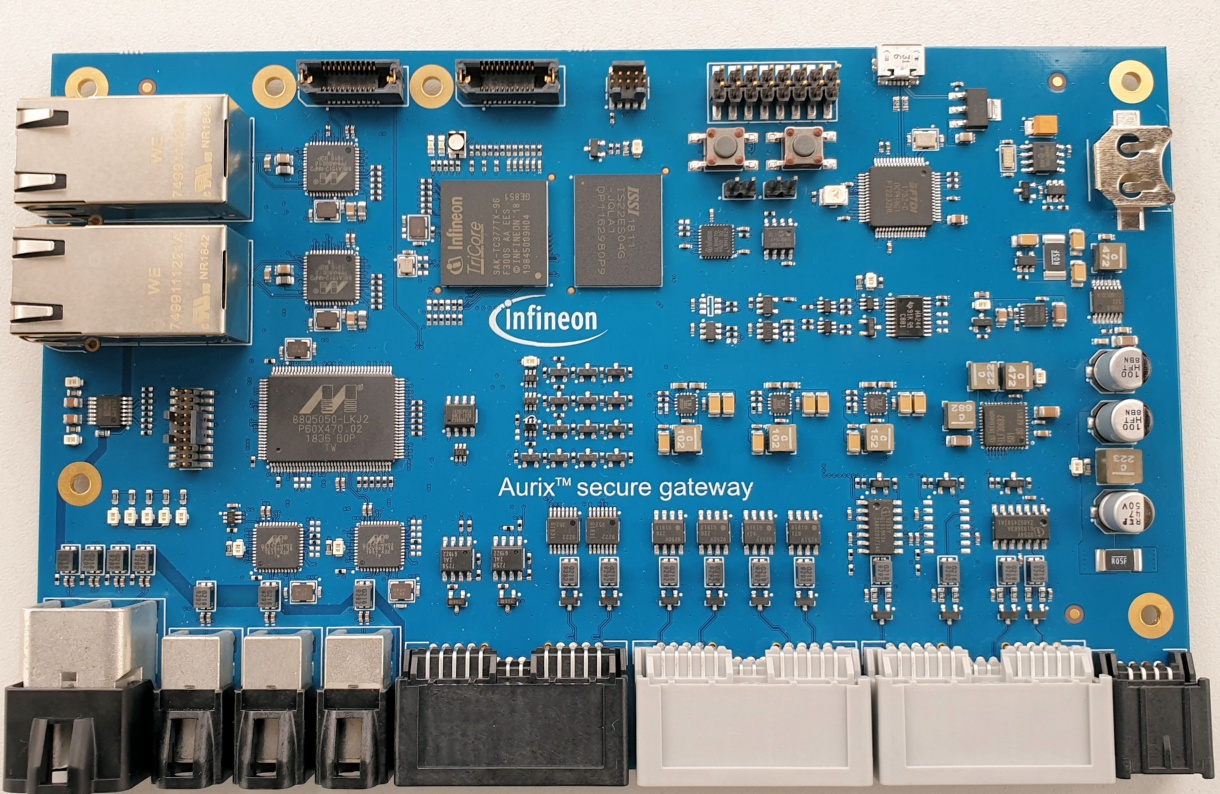
\includegraphics[width=0.8\textwidth]{img/secure-gateway.jpg}
 \caption{KIT\_A2G\_TC377\_SEC\_GTW}
 \label{fig:gw-photo}
\end{figure}

\begin{figure}[!htb]
 \centering
 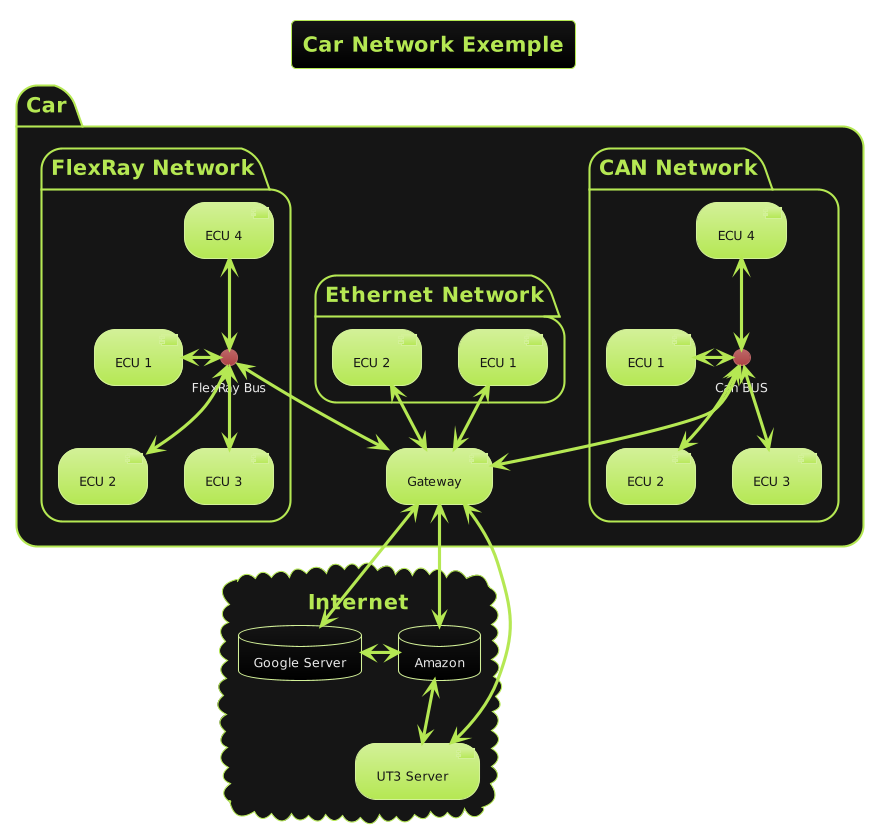
\includegraphics[width=\textwidth]{img/gateway_car.png}
 \caption{Exemple des réseaux interconnect\'ees dans une voiture}
 \label{fig:gw-car}
\end{figure}

\begin{figure}[!htb]
 \centering
 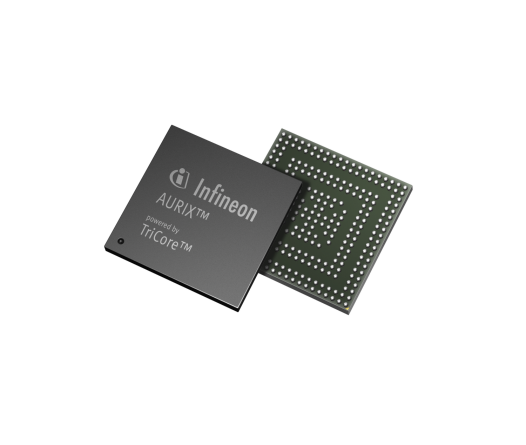
\includegraphics[width=0.5\textwidth]{img/Aurix.png}
 \caption{AURIX (Automotive Realtime Integrated NeXt Generation Architecture)}
 \label{fig:aurix-photo}
\end{figure}

Le système d'exploitation est fourni avec une petite démo technique qui sert pour la prise en main de la Gateway et tester son fonctionnement basique de connecter 2 réseaux avec des protocoles physiques et logiques incompatibles. Pour lancer la démo il est nécessaire de connecter 2 ECU externes \`a certains ports CAN et Ethernet du Gateway, voir figures \ref{fig:gw-demo-uc1} et \ref{fig:gw-demo-uc2} pour plus d'information concernant aux connections. La démo a 2 cas d'utilisation : 

\begin{itemize} 

    \item Use Case 1 : L'ECU connect\'e au port CAN envoie une trame d'information qui sera renvoyée vers l'ECU en Ethernet (fig. \ref{fig:gw-demo-uc1}). 

    \item Use Case 2 : L'ECU connect\'e au port Ethernet envoie une trame d'information qui sera renvoyée vers l'ECU en CAN (fig. \ref{fig:gw-demo-uc2}). 

\end{itemize} 

\begin{figure}[!htb]
 \centering
 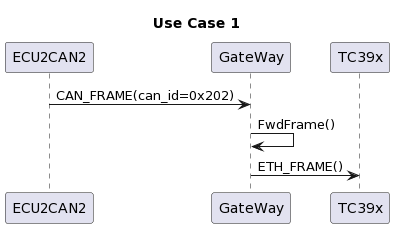
\includegraphics[width=0.6\textwidth]{img/GWUseCase1.png}
 \caption{Gateway Demo Use Case 1}
 \label{fig:gw-demo-uc1}
\end{figure}

\begin{figure}[!htb]
 \centering
 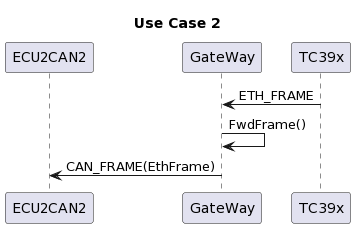
\includegraphics[width=0.7\textwidth]{img/GWUseCase2.png}
 \caption{Gateway Demo Use Case 2}
 \label{fig:gw-demo-uc2}
\end{figure}

Pour tester le fonctionnement basique de cette Gateway il nous faut toute une infrastructure comme une réseaux CAN, des ECU compatibles, un banc de tests, outils de vérification, etc, ce nous présente les problèmes suivants : 

\begin{itemize} 

    \item Construction d'un espace contrôlé et sécurisé pour accueillir ces composants. 

    \item Haute coûte d'achats des composants pour tester qui pourront ne pas être disponibles vu la situation actuelle des semiconducteurs. 

    \item Fabrication des bancs de test. 

    \item Frais des maintenances future pour maintenir le bon fonctionnement du banc de test.   

\end{itemize} 

Toutes ces problèmes augmentent le co\^ut et la durée du projet, et si les besoins du projet changent il sera nécessaire changer des composants ou fabriquer des nouvelles pièces de hardware. Dans une cadre du développement de logiciel ce n'est pas le cas le plus efficace. 

\subsection{Objectifs du projet} 

  

ASTC Design Partners veut virtualiser cette Gateway en utilisant son outil VLAB Works. Avec une solution virtualis\'ee non seulement les coûts de fabrication, délais de livraison et maintenance seront évités mais aussi le développement de tests automatises sera plus rapide, chaque développeur aura son propre banc de test personnalisés et les bugs software seront trouvés plus facilement.  

Au début du projet nous avions disponible VLAB, la modèle virtualis\'ee du microcontrôleur \textit{AURIX TC37x} utilisée dans la Gateway et le software compil\'e MICROSAR fournie avec la Gateway. Le software de la Gateway doit vérifier le fonctionnement correct de toutes les composants et buses de données présents sur la Gateway. Afin de virtualiser la Gateway, il faut remplir quelques objectifs basiques :  

\begin{itemize} 

    \item - Modéliser des composants nécessaires pour que le système d'exploitation démarre. 

    \item - Faire un testbench avec les bus de donn\'ees nécessaires pour l'envoie des donn\'ees. 

    \item - Augmenter les capacit\'es du \textit{TC37x} parce que la Gateway utilise une version amelior\'e de ce microcontr\^oleur appelée par Infineon \textit{TC37xEXT}\cite{aurix.tc37e}. 

\end{itemize} 